\chapter{Perceptron}
\label{chap:Perceptron}

\section{Model}
\begin{equation}
\mathcal{H}:f(\vec{x})=\text{sign}(\vec{w}\vec{x}+b)
\end{equation}
where $\text{sign}(x)=\begin{cases}+1, & x \geq 0\\-1, & x<0\\\end{cases}$, see Fig. ~\ref{fig:perceptron}\footnote{\url{https://en.wikipedia.org/wiki/Perceptron}}.
\begin{figure}[hbtp]
\centering
    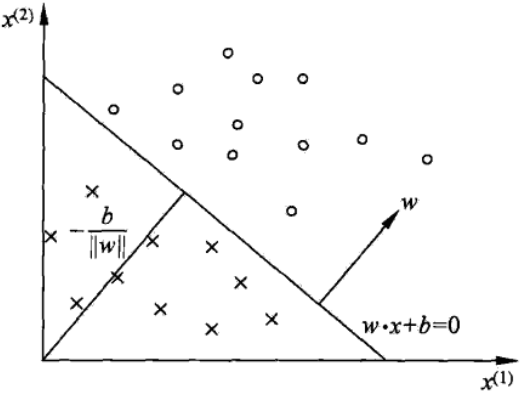
\includegraphics[scale=.50]{figures/perceptron.png}
\caption{Perceptron}
\label{fig:perceptron} 
\end{figure}

Perceptron is a binary linear classifier, which is a discriminant model.

\section{Strategy}
\begin{eqnarray}
L(\vec{w},b)&=&-y_i(\vec{wx}_i+b)\\
R_{emp}(f)&=&-\sum\limits_i y_i(\vec{wx}_i+b)\\
\end{eqnarray}

\section{Learning algorithm}
\subsection{Primal form}
Stochastic gradient descent, the pseudo code is as follows:
\begin{algorithm}[htbp]
    %\SetAlgoLined
    \SetAlgoNoLine
  
    $\vec{w} \leftarrow 0;\; b \leftarrow 0;\; k \leftarrow 0$\;
    \While{no mistakes made within the for loop}{
        \For{$i\leftarrow 1$ \KwTo $N$}{
			\If{$y_i(\vec{w}^T\vec{x}_i+b) \leq 0$}{
				$\vec{w} \leftarrow \vec{w}+\eta y_i \vec{x}_i$\;
				$b \leftarrow b+\eta y_i$\;
				$k \leftarrow k+1$\;
			}
		}
    }
\caption{Perceptron learning algorithm, primal form}
\end{algorithm}

\subsection{Convergency}
\begin{theorem}
(\textbf{Novikoff}) If traning data set $\mathcal{D}$ is linearly separable, then
\begin{enumerate}
\item There exists a hyperplane denoted as $\widehat{\vec{w}}_{opt} \cdot \vec{x}+b_{opt}=0$ which can correctly seperate all samples, and 
\begin{equation}
\exists\gamma>0,\forall i, y_i(\vec{w}_{opt} \cdot \vec{x}_i+b_{opt}) \geq \gamma
\end{equation}
\item \begin{equation}k \leq \left(\dfrac{R}{\gamma}\right)^2,\text{ where } R=\max\limits_{1 \leq i \leq N} \abs{\abs{\widehat{\vec{x}}_i}}
\end{equation}

\end{enumerate}
\end{theorem}

\begin{proof}
(1) let $\gamma=\min\limits_{i} y_i(\vec{w}_{opt} \cdot \vec{x}_i+b_{opt})$, then we get $y_i(\vec{w}_{opt} \cdot \vec{x}_i+b_{opt}) \geq \gamma$.

(2) The algorithm start from $\widehat{\vec{x}}_0=0$, if a instance is misclassified, then update the weight. Let $\widehat{\vec{w}}_{k-1}$ denotes the extended weight before the k-th misclassified instance, then we can get
\begin{eqnarray}
y_i(\widehat{\vec{w}}_{k-1} \cdot \widehat{\vec{x}_i})&=&y_i(\vec{w}_{k-1} \cdot \vec{x}_i+b_{k-1}) \leq 0\\
\widehat{\vec{w}}_k&=&\widehat{\vec{w}}_{k-1}+\eta y_i \widehat{\vec{x}_i}
\end{eqnarray}

We could infer the following two equations, the proof procedure are omitted.
\begin{enumerate}
\item $\widehat{\vec{w}}_k \cdot \widehat{\vec{w}}_{opt} \geq k\eta\gamma$
\item $\abs{\abs{\widehat{\vec{w}}_k}}^2 \leq k\eta^2R^2$
\end{enumerate}

From above two equations we get
\begin{eqnarray}
\nonumber k\eta\gamma & \leq & \widehat{\vec{w}}_k \cdot \widehat{\vec{w}}_{opt} \leq \abs{\abs{\widehat{\vec{w}}_k}}\abs{\abs{\widehat{\vec{w}}_{opt}}} \leq \sqrt k \eta R \\
\nonumber k^2\gamma^2 & \leq & kR^2 \\
\nonumber \text{i.e. } k & \leq & \left(\dfrac{R}{\gamma}\right)^2
\end{eqnarray}
\end{proof}

\subsection{Dual form}
\begin{eqnarray}
\vec{w}&=&\sum\limits_{i=1}^{N} \alpha_iy_i\vec{x}_i \\
b&=&\sum\limits_{i=1}^{N} \alpha_iy_i \\
f(\vec{x})&=&\text{sign}\left(\sum\limits_{j=1}^{N} \alpha_jy_j\vec{x}_j \cdot \vec{x}+b\right)
\end{eqnarray}

\begin{algorithm}[htbp]
    %\SetAlgoLined
    \SetAlgoNoLine
  
    $\vec{\alpha} \leftarrow 0;\; b \leftarrow 0;\; k \leftarrow 0$\;
    \While{no mistakes made within the for loop}{
        \For{$i\leftarrow 1$ \KwTo $N$}{
			\If{$y_i\left(\sum\limits_{j=1}^{N} \alpha_jy_j\vec{x}_j \cdot \vec{x}_i+b\right) \leq 0$}{
				$\vec{\alpha} \leftarrow \vec{\alpha}+\eta$\;
				$b \leftarrow b+\eta y_i$\;
				$k \leftarrow k+1$\;
			}
		}
    }
\caption{Perceptron learning algorithm, dual form}
\end{algorithm}